
\documentclass{article}
\usepackage[utf8]{inputenc}
\usepackage{mathtools}
\usepackage{amssymb}
\usepackage{amsmath}
\usepackage{listings}
\usepackage{braket}

%%%THEOREM (ETC) ENVIRONMENTS
\newtheorem{theorem}{Theorem}[section]
\newtheorem{lemma}[theorem]{Lemma}
\newtheorem{proposition}[theorem]{Proposition}
\newtheorem{corollary}[theorem]{Corollary}

\newenvironment{proof}[1][Proof]{\begin{trivlist}
\item[\hskip \labelsep {\bfseries #1}]}{\end{trivlist}}
\newenvironment{definition}[1][Definition]{\begin{trivlist}
\item[\hskip \labelsep {\bfseries #1}]}{\end{trivlist}}
\newenvironment{example}[1][Example]{\begin{trivlist}
\item[\hskip \labelsep {\bfseries #1}]}{\end{trivlist}}
\newenvironment{remark}[1][Remark]{\begin{trivlist}
\item[\hskip \labelsep {\bfseries #1}]}{\end{trivlist}}

\newcommand{\Tau}{\mathrm{T}}
\newcommand{\ham}{\mathcal{H}}

\title{Categorical Semantics for Topological Quantum Computation}
\author{Giovanni de Felice}
\date{April 2017}

%%%TIKZ:
\usepackage{tikz,pgfplots}
\usetikzlibrary{shapes.geometric}
\usetikzlibrary{trees, patterns}
\usetikzlibrary{positioning}
\usepackage{tikz,ifthen,calc}
\usepackage{tkz-euclide}
\usetikzlibrary{shapes,snakes}
\usetikzlibrary{calc,intersections, fit, knots, hobby, positioning, patterns}
\usepackage{braids}

%%%categorical diagrams:
\tikzset{
	buffer/.style={
		draw,
		shape border rotate=180,
		regular polygon,
		regular polygon sides=3,
		node distance=2cm,
		minimum height=4em
	}
}
%%%HOPF ALGEBRAS:
\newcommand{\mult}{
	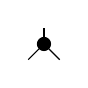
\begin{tikzpicture}[scale=0.2, black/.style={scale=0.5,draw,shape=circle,fill=black}]
	\node[black] (0) at (0, 0) {};
	\draw (1,-1) to (0);
	\draw (-1,-1) to (0);
	\draw (0) to (0,1);
	\end{tikzpicture}
}
\newcommand{\unit}{
	
\begin{tikzpicture}[scale=0.2, black/.style={scale=0.5,draw,shape=circle,fill=black}]
	\node[black] (0) at (0, 0) {};
	\draw (0) to (0,1);
	\end{tikzpicture}
}
\newcommand{\comult}{
	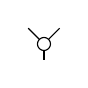
\begin{tikzpicture}[scale=0.2, black/.style={scale=0.5,draw,shape=circle,fill=white}]
	\node[black] (0) at (0, 0) {};
	\draw (1,1) to (0);
	\draw (-1,1) to (0);
	\draw (0) to (0,-1);
	\end{tikzpicture}
}

\newcommand{\counit}{
	\begin{tikzpicture}[scale=0.2, black/.style={scale=0.5,draw,shape=circle,fill=white}]
	\node[black] (0) at (0, 0) {};
	\draw (0) to (0,-1);
	\end{tikzpicture}
}

\newcommand{\antipode}{
	\begin{tikzpicture}[scale=0.2, black/.style={scale=0.5,draw,regular polygon,
		regular polygon sides=4,fill=white}]
	\node[black] (0) at (0, 0) {};
	\draw (0) to (0,-1);
	\draw (0) to (0,1);
	\end{tikzpicture}
}

\newcommand{\associativity}{
\begin{equation}
\begin{gathered}
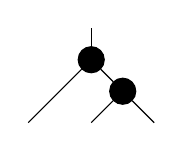
\begin{tikzpicture}[scale=0.8]
\node[draw,circle,fill=black] (0) at (0,0.5) {};
\node[draw,circle,fill=black] (1) at (0.5,0) {};
\draw (0) to (1);
\draw (-1,-0.5) to (0);
\draw (0,-0.5) to (1);
\draw (1,-0.5) to (1);
\draw (0) to (0,1);
\end{tikzpicture}
\end{gathered}
\, = \,
\begin{gathered}
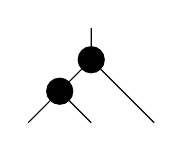
\begin{tikzpicture}[scale=0.8]
\node[draw,circle,fill=black] (0) at (0.5,0.5) {};
\node[draw,circle,fill=black] (1) at (0,0) {};
\draw (0) to (1);
\draw (-0.5,-0.5) to (1);
\draw (0.5,-0.5) to (1);
\draw (1.5,-0.5) to (0);
\draw (0) to (0.5,1);
\end{tikzpicture}
\end{gathered}
\end{equation}
}
\newcommand{\unitlaw}{
\begin{equation}
\begin{gathered}
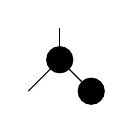
\begin{tikzpicture}[scale=0.8]
\node[draw,circle,fill=black] (0) at (0,0.5) {};
\node[draw,circle,fill=black] (1) at (0.5,0) {};
\draw (0) to (1);
\draw (-0.5,0) to (0);
\draw (0) to (0,1);
\end{tikzpicture}
\end{gathered}
\, = \,
\begin{gathered}
\begin{tikzpicture}[scale=0.8]
\draw (0,0) to (0,1);
\end{tikzpicture}
\end{gathered}
\, = \,
\begin{gathered}
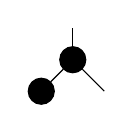
\begin{tikzpicture}[scale=0.8]
\node[draw,circle,fill=black] (0) at (0,0.5) {};
\node[draw,circle,fill=black] (1) at (-0.5,0) {};
\draw (0) to (1);
\draw (0.5,0) to (0);
\draw (0) to (0,1);
\end{tikzpicture}
\end{gathered}
\end{equation}
}
\newcommand{\coassociativity}{
\begin{equation}
\begin{gathered}
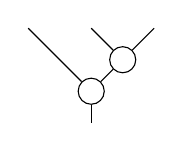
\begin{tikzpicture}[scale=0.8]
\node[draw,circle,fill=white] (0) at (0,-0.5) {};
\node[draw,circle,fill=white] (1) at (0.5,0) {};
\draw (0) to (1);
\draw (-1,0.5) to (0);
\draw (0,0.5) to (1);
\draw (1,0.5) to (1);
\draw (0) to (0,-1);
\end{tikzpicture}
\end{gathered}
\, = \,
\begin{gathered}
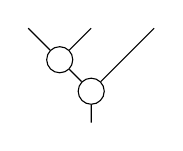
\begin{tikzpicture}[scale=0.8]
\node[draw,circle,fill=white] (0) at (0.5,-0.5) {};
\node[draw,circle,fill=white] (1) at (0,0) {};
\draw (0) to (1);
\draw (-0.5,0.5) to (1);
\draw (0.5,0.5) to (1);
\draw (1.5,0.5) to (0);
\draw (0) to (0.5,-1);
\end{tikzpicture}
\end{gathered}
\end{equation}
}
\newcommand{\counitlaw}{
\begin{equation}
\begin{gathered}
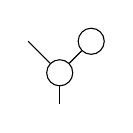
\begin{tikzpicture}[scale=0.8]
\node[draw,circle,fill=white] (0) at (0,-0.5) {};
\node[draw,circle,fill=white] (1) at (0.5,0) {};
\draw (0) to (1);
\draw (-0.5,0) to (0);
\draw (0) to (0,-1);
\end{tikzpicture}
\end{gathered}
\, = \,
\begin{gathered}
\begin{tikzpicture}[scale=0.8]
\draw (0,0) to (0,1);
\end{tikzpicture}
\end{gathered}
\, = \,
\begin{gathered}
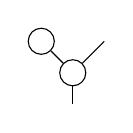
\begin{tikzpicture}[scale=0.8]
\node[draw,circle,fill=white] (0) at (0,-0.5) {};
\node[draw,circle,fill=white] (1) at (-0.5,0) {};
\draw (0) to (1);
\draw (0.5,0) to (0);
\draw (0) to (0,-1);
\end{tikzpicture}
\end{gathered}
\end{equation}
}

\newcommand{\bialgebralaw}{
\begin{equation}
\begin{gathered}
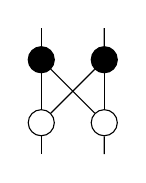
\begin{tikzpicture}[scale=0.8]
\node[draw,circle,fill=white] (0) at (0,0) {};
\node[draw,circle,fill=white] (1) at (1,0) {};
\node[draw,circle,fill=black] (2) at (0,1) {};
\node[draw,circle,fill=black] (3) at (1,1) {};
\draw (0) to (2);
\draw (0) to (3);
\draw (1) to (2);
\draw (1) to (3);
\draw (0,-0.5) to (0);
\draw (1,-0.5) to (1);
\draw (0,1.5) to (2);
\draw (1,1.5) to (3);
\end{tikzpicture}
\end{gathered}
\, = \,
\begin{gathered}
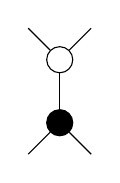
\begin{tikzpicture}[scale=0.8]
\node[draw,circle,fill=black] (0) at (0.5,0) {};
\node[draw,circle,fill=white] (1) at (0.5,1) {};
\draw (0) to (1);
\draw (0,-0.5) to (0);
\draw (1,-0.5) to (0);
\draw (0,1.5) to (1);
\draw (1,1.5) to (1);
\end{tikzpicture}
\end{gathered}
\end{equation}
}
\newcommand{\hopflaw}{
	\begin{equation}
	\begin{gathered}
	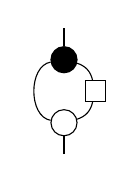
\begin{tikzpicture}[scale=0.8, squr/.style={draw,regular polygon,
		regular polygon sides=4,fill=white}]
	\node[draw,circle,fill=white] (0) at (0,0) {};
	\node[draw,circle,fill=black] (1) at (0,1) {};
	\node[scale=0.8,squr] (2) at (0.5,0.5) {};
	\draw[bend left=80] (0) to (1);
	\draw[bend right] (0) to (2);
	\draw[bend right] (2) to (1);
	\draw (0,-0.5) to (0);
	\draw (0,1.5) to (1);
	\end{tikzpicture}
	\end{gathered}
	\, = \,
	\begin{gathered}
	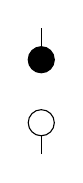
\begin{tikzpicture}[scale=0.8, squr/.style={draw,regular polygon,
		regular polygon sides=4,fill=white}]
	\node[draw,circle,fill=white] (0) at (0,0) {};
	\node[draw,circle,fill=black] (1) at (0,1) {};
	\draw (0,-0.5) to (0);
	\draw (0,1.5) to (1);
	\end{tikzpicture}
	\end{gathered}
	\end{equation}
}

\newcommand{\symAB}{
	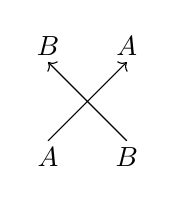
\begin{tikzpicture}[decoration={markings,mark=at position 0.5 with {\arrow{>}}}]
	\node (0) at (-0.5, -0.7) {$A$};
	\node (0) at (-0.5, 0.7) {$B$};
	\node (1) at (0.5, -0.7) {$B$};
	\node (1) at (0.5, 0.7) {$A$};
	\draw [->] (-0.5, -0.5) to (0.5, 0.5);
	\draw [->] (0.5, -0.5) to (-0.5, 0.5);
	\end{tikzpicture}
}

\newcommand{\symequation}{
	\begin{equation*}
	\begin{gathered}
	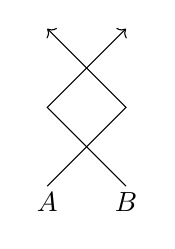
\begin{tikzpicture}
	\node (0) at (-1, -1.2) {$A$};
	\node (0) at (0, -1.2) {$B$};
	\draw [->] (-1, -1)--(0,0)--(-1,1);
	\draw [->] (0, -1)--(-1,0)--(0,1);
	\end{tikzpicture}
	\end{gathered}
	\, = \,
	\begin{gathered}
	\begin{tikzpicture}
	\node (0) at (-0.8, -1.2) {$A$};
	\node (0) at (0, -1.2) {$B$};
	\draw [->] (-0.8, -1)--(-0.8,1);
	\draw [->] (0, -1)--(0,1);
	\end{tikzpicture}
	\end{gathered}
	\end{equation*}
}

\newcommand{\cupA}{	
	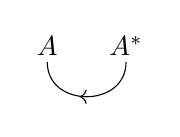
\begin{tikzpicture}[decoration={markings,mark=at position 0.5 with {\arrow{<}}}]
	\node (0) at (0, 0.2) {$A$};
	\node (1) at (1, 0.2) {$A^*$};
	\draw [bend right=90, looseness=1.5, postaction=decorate] (0,0) to (1,0);
	\end{tikzpicture}}

\newcommand{\capA}{	
	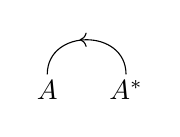
\begin{tikzpicture}[decoration={markings,mark=at position 0.5 with {\arrow{<}}}]
	\node (0) at (0, -0.2) {$A$};
	\node (1) at (1, -0.2) {$A^*$};
	\draw [bend left=90, looseness=1.5, postaction=decorate] (0,0) to (1,0);
	\end{tikzpicture}}

\newcommand{\snake}{
	\begin{equation*}
	\begin{gathered}
	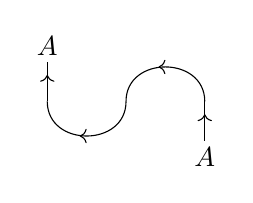
\begin{tikzpicture}[decoration={markings,mark=at position 0.5 with {\arrow{<}}}]
	\node (0) at (0, 0.7) {$A$};
	\node (4) at (2, -0.7){$A$};
	\draw [bend right=90, looseness=1.5, postaction=decorate] (0, 0) to (1, 0);
	\draw [bend left=90, looseness=1.5, postaction=decorate] (1, 0) to (2, 0);
	\draw [postaction=decorate] (2, 0) to (2, -0.5);
	\draw [postaction=decorate] (0, 0.5) to (0, 0);
	\end{tikzpicture}
	\end{gathered}
	\, = \,
	\begin{gathered}
	\begin{tikzpicture}[decoration={markings,mark=at position 0.5 with {\arrow{<}}}]
	\node (0) at (0, 0.7) {$A$};
	\node (4) at (0, -0.7){$A$};
	\draw [postaction=decorate] (0, 0.5) to (0, -0.5);
	\end{tikzpicture}
	\end{gathered}
	\end{equation*}}

\newcommand{\snakestar}{
	\begin{equation*}
	\begin{gathered}
	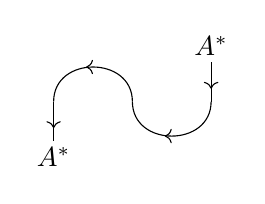
\begin{tikzpicture}[decoration={markings,mark=at position 0.5 with {\arrow{<}}}]
	\node (0) at (0, -0.7) {$A^*$};
	\node (4) at (2, 0.7){$A^*$};
	\draw [bend left=90, looseness=1.5, postaction=decorate] (0, 0) to (1, 0);
	\draw [bend right=90, looseness=1.5, postaction=decorate] (1, 0) to (2, 0);
	\draw [postaction=decorate] (2, 0) to (2, 0.5);
	\draw [postaction=decorate] (0, -0.5) to (0, 0);
	\end{tikzpicture}
	\end{gathered}
	\, = \,
	\begin{gathered}
	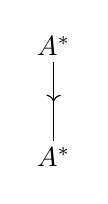
\begin{tikzpicture}[decoration={markings,mark=at position 0.5 with {\arrow{>}}}]
	\node (0) at (0, 0.7) {$A^*$};
	\node (4) at (0, -0.7){$A^*$};
	\draw [postaction=decorate] (0, 0.5) to (0, -0.5);
	\end{tikzpicture}
	\end{gathered}
	\end{equation*}
}

\newcommand{\fusionijk}{
	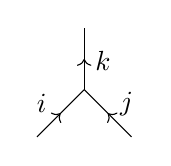
\begin{tikzpicture}[scale=0.6,decoration={markings,mark=at position 0.5 with {\arrow{>}}}]
	\node (0) at (-0.9, -0.3) {$i$};
	\node (1) at (0.9, -0.3) {$j$};
	\node (2) at (0.4, 0.6) {$k$};
	\draw [postaction=decorate] (-1, -1) to(0,0);
	\draw [postaction=decorate] (1,-1) to (0,0);
	\draw [postaction=decorate] (0,0) to (0,1.3);
	\end{tikzpicture}}
%%%%%%%%%%%%%%%%%%%%%%%%%%%%%%%%%%%%%%%%%%%%%%%%%%%%%%%%%%%%%%%%%%%%%%%%%%%%%%%%%%%%%%%%%%%%%%%%%%%%%%%%%%%%%%%%%%%%%%%%%%%%%%%%%%%%%%%%%%%%%%%%%%%%%%%%%%%%%%%%%%%%%%%%%%%%%%%%%%%%


\begin{document}
\maketitle
\tableofcontents

\pagebreak
\section{Introduction}
Categories and diagrams \\
Symmetry, quantization and categorification\\
Categorification = replacing equalities with isomorphisms\\
quantization =\\
Mathematically: from groups to quasitriangular hopf algebras, G to DG\\
Categorically: from symmetric fusion categories to modular categories\\
Physically: fermions/bosons to anyons, local symmetries to topological symmetries, 3D to 2D\\
Computation: from PQC to TQC, complexity theory\\
Logic: mirror the relationship, all statements about RepDG are statements in RepG, a modality, programming language
\begin{definition}
categories, functors, natural transformations
\end{definition}
\section{Representation Theory}
%%%%%%%%%%%%%%%%%%%%%%%%%%%%%%%%%%%%%%%%%%%%%%%%%%%%%%%%%%%%%%%%%%%%%%%%%%%%%%%%%%%%%%%%%%%%%%%%%%%%%%%%%%%%%%%%%%%%%%%%%%%%%%%%%%%%%%%%%%%%%%%%
%%%%%%%%%%%%%%%%%%%%%%%%%%%%%%%%%%%%%%%%%%%%%%%%%%%%%%%%%%%%%%%%%%%%%%%%%%%%%%%%%%%%%%%%%%%%%%%%%%%%%%%%%%%%%%%%%%%%%%%%%%%%%%%%%%%%%%%%%%%%%%%%
\subsection{Monoidal categories}
In this section, we set in place the basic definitions and diagrammatic  intuitions which we will use throughout the thesis.\\
%%CATEGORIES:
Recall that a category is a collection of objects and arrows such that arrows compose in the sense if $f$ and $g$ are arrows as below then there is an arrow $g \circ f$ as follows: 	
\begin{center}
	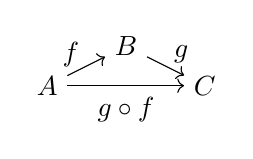
\begin{tikzpicture}
	\node (0) at (-1, 0) {$A$};
	\node (1) at (0, 0.5) {$B$};
	\node (2) at (1, 0) {$C$};
	\node (3) at (-0.7, 0.4) {$f$};
	\node (3) at (0.7, 0.4) {$g$};
	\node (3) at (0, -0.3) {$g\circ f$};
	\draw [->] (0) to (1);
	\draw [->] (1) to (2);
	\draw [->] (0) to (2);
	\end{tikzpicture}
\end{center}
The above diagram is a statement about categories, and it has exactly the same information to its dual diagram. Where objects are one-dimensional wires and morphisms are one dimensional cells:
\begin{center}
	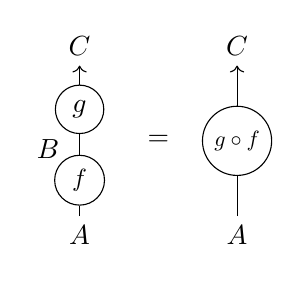
\begin{tikzpicture}
	\node (0) at (-1, -1.2) {$A$};
	\node (1) at (-1.4, -0.1) {$B$};
	\node (2) at (-1, 1.2) {$C$};
	\node (3) at (1, -1.2) {$A$};
	\node (4) at (1, 1.2) {$C$};
	\node[scale=0.9,draw,circle] (5) at (-1, -0.5) {$f$};
	\node[draw,circle] (6) at (-1, 0.4) {$g$};
	\node[scale=0.8,draw,circle] (7) at (1, 0) {$g\circ f$};
	\node (8) at (0, 0) {$=$};
	\draw (0) to (5);
	\draw (5) to (6);
	\draw [->] (6) to (2);
	\draw (3) to (7);
	\draw [->] (7) to (4);
	\end{tikzpicture}
\end{center}
Category theory is a really good language for talking about equivalences and relationships between structures.
Given two categories $\mathcal{C}$ and $\mathcal{D}$ a functor $F: \mathcal{C} \rightarrow \mathcal{D}$ is a transformation taking objects of $\mathcal{C}$ to objects of $\mathcal{D}$ and arrows to arrows preserving the inner structure of the category (i.e identity arrows and composition).
\begin{definition}
	A functor $F:\mathcal{C} \rightarrow \mathcal{D}$ is a mapping that
	\begin{itemize}
		\item associates an object $F(X)$ of $\mathcal{D}$ to each object $X$ of $\mathcal{C}$.
		\item associates to each morphism $f:X \rightarrow Y$ a morphism $F(f): F(X) \rightarrow F(Y)$ such that $F(id_X)=id_Y$ and $F(g\circ f)= F(g)\circ F(f)$ for all morphisms $f:X \rightarrow Y$ and $g:Y \rightarrow Z$.
	\end{itemize}
\end{definition}For instance there is a functor $Q: Sets \rightarrow Hilb$ called `1st quantization' and taking a set to the free hilbert space generated by that set. It is easy to see that $Q$ also preserves the monoidal structure as well as the symmetry morphisms, we say $Q$ is a symmetric monoidal functor.
%%%MONOIDAL CATEGORIES:
Recall that a monoid is a triple $(X, \times, 1)$ where $X$ is a set, $1 \in X$ and $\times$ is an associative and unital multiplication on $X$. The notion of a monoidal category is the categorification of a monoid. Elements of the set are replaced by objects in a category $\mathcal{C}$, multiplication by a bifunctor $\otimes: \mathcal{C} \times \mathcal{C} \rightarrow \mathcal{C}$ and the equalities in the unit and association axioms are replaced by natural isomorphisms. In order for this new structure to be well-behaved we will also need to impose compatibility conditions.
We obtain the following definition:
\begin{definition}
A monoidal category is a quintuple $(\mathcal{C}, \otimes, 1, a, i)$ where $\mathcal{C}$ is a category, $\otimes: \mathcal{C} \times \mathcal{C} \rightarrow \mathcal{C}$ is a bifunctor called tensor product.
$$ a : -\otimes(- \otimes -) \xrightarrow{\sim} (-\otimes -) \otimes -$$ is a natural isomorphism. $1$ is an object of $\mathcal{C}$ subject to the following axioms:
\begin{enumerate}
    \item Pentagon axiom: the following diagram commutes for all objects $W,X,Y,Z$ in $\mathcal{C}$.
    \item Unit axiom: the left and right unitors are equivalences $\mathcal{C} \rightarrow \mathcal{C}$.
\end{enumerate}
\end{definition}
Let us give three important examples of monoidal categories.
\begin{example}
The category $Sets$ of sets and functions is monoidal with the cartesian product $\times$ as bifunctor and the singleton set as unit object.\\
The category $Vect_k$ of vector spaces over a field $k$ is monoidal with the usual tensor product $\otimes$ and the one dimensional vector space $k$ as unit object.\\
The category $Rel$ of sets and relations is monoidal with the cartesian product $\times$ and the singleton as unit object.
\end{example}

The more structure comes with a category the more complicated diagrams we can draw. For the moment our diagrams can only be one dimensional because we have only one notion of composition. Monoidal categories are categories $\mathcal{C}$ equipped with a bifunctor $\otimes : \mathcal{C} \times \mathcal{C} \rightarrow \mathcal{C}$, a unit object $I$ and natural unitors and associators satisfying certain coherence conditions. The rigorous definition can be found in [maclane]. Monoidal categories have a two-dimensional diagrammatic language. The presence of unitors and associators and the conditions they satisfy make sure that this graphical language is well behaved. We write the tensor of two morphisms $f \otimes g : A \otimes B \rightarrow C \otimes D$ simply putting them side by side:
\begin{center}
	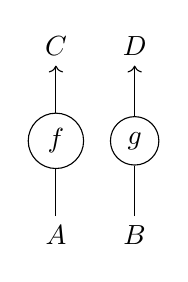
\begin{tikzpicture}
	\node (0) at (0, -1.2) {$A$};
	\node (1) at (1, -1.2) {$B$};
	\node (2) at (0, 1.2) {$C$};
	\node (3) at (1, 1.2) {$D$};
	\node[draw,circle] (5) at (0, 0) {$f$};
	\node[draw,circle] (6) at (1, 0) {$g$};
	\draw (0) to (5);
	\draw [->] (5) to (2);
	\draw (1) to (6);
	\draw [->] (6) to (3);
	\end{tikzpicture}
\end{center}
In our diagrams we can picture the unit $I$ of the tensor as the plane on which we are drawing. Indeed we could imagine drawing as many copies as we wanted of $id_I$ on the previous diagram to obtain obtain an equivalent diagram as $id_I \otimes f = f$ for any morphism $f$. So really the identity on $I$ is just the empty diagram which we can stick next to any diagram we like. Processes from the unit $I$ to some object $A$ are called `states' of $A$ and we draw them as follows:
\begin{center}
	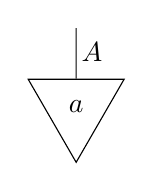
\begin{tikzpicture}
	\node[buffer] (1) {$a$}; 
	\node (2) at (0.2,0.7) {$A$};
	\draw (1)--(0,1);
	\end{tikzpicture}
\end{center}

%%%DIAGRAMS:
The above is the classical introduction to monoidal categories as a category with some extra structure. Monoidal categories can also be seen as degenerate 2-categories. Although this viewpoint requires one additional initial step of abstraction (the definition of a 2-category), we will see that it will give us the diagrammatic language for monoidal categories for free. For the rigorous definition of a 2-category we refer to [BAEZ], for our purposes we will only need the intuition. A 2-category is a collection of objects with 1-arrows between them and 2-arrows between the 1-arrows. Note that there are two ways of composing the 2-arrows, vertically and horizontally. (DIAGRAMS-...) Taking the dual diagrams we obtain the diagrammatic language. Monoidal categories are 2-categories with only one 0-object called $1$. We can think of it as the underlying plane or the empty diagram, wires carry systems (1-arrows), boxes are morphisms (2-arrows). We recover the given definition of monoidal category by calling 1-arrow objects, and 2-arrows morphisms. The unit object $1$ is then the identity 1-arrow $1 \rightarrow 1$ which we will denote by $1$. 
\begin{definition}
Given a system $A$, a state of is a morphism $1 \rightarrow A$. A costate (or effect) of $A$ is a morphism $A \rightarrow 1$. We denote them as folows in the diagrammatic language.
\end{definition}
\begin{example}
The category $Sets$ of sets and functions has monoidal structure given by the Cartesian product of sets. The product $A \times B$ of sets $A$ and $B$, satisfies the universal properties of a categorical product, in the sense that we have projections $p_1$ and $p_2$ such that if $f$ and $g$ are maps from some set $C$ there is a unique function $h$ making the following diagram commute:
\begin{center}
	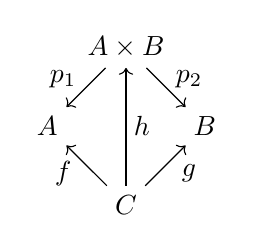
\begin{tikzpicture}
	\node (0) at (-1, 0) {$A$};
	\node (1) at (1, 0) {$B$};
	\node (2) at (0, 1) {$A \times B$};
	\node (3) at (0, -1) {$C$};
	\node (4) at (0.2, 0) {$h$};
	\node (5) at (-0.8, 0.6) {$p_1$};
	\node (6) at (0.8, 0.6) {$p_2$};
	\node (7) at (-0.8, -0.6) {$f$};
	\node (8) at (0.8, -0.6) {$g$};
	\draw [->] (2) to (0);
	\draw [->] (2) to (1);
	\draw [->] (3) to (1);
	\draw [->] (3) to (0);
	\draw [->] (3) to (2);
	\end{tikzpicture}
\end{center}
Because of this property all states of $(Sets,\times)$ are separable. This category is the ambient Cartesian world of classical physics.
\end{example}
\begin{example}
In $Vect_k$ states are vectors and costates are functionals. Note that the diagrammatic notation provides a two-dimensional generalisation of Dirac's notation. The category $Hilb$ of Hilbert spaces and linear maps is monoidal when equipped with the usual tensor product $\otimes$. Note that $\otimes$ is not a categorical product, and in fact we can have entangled states. Quantum mechanics is based on $(Hilb, \otimes)$ as shown by Vicary [categorical quantum notes].
\end{example}

\begin{definition}
Scalars in a monoidal category are morphisms $1 \rightarrow 1$.
\end{definition}
The category $Sets$ has only one scalar. $Rel$ has two scalars forming the cyclic group $\mathbb{Z}_2$ under composition. $Vect_k$ has scalars from $k$. Given a vector and a functional we obtain a scalar by composing them analogously to Dirac's formalism.\\
Both $Sets$ and $Hilb$ are examples of symmetric monoidal categories.In the sense that  any pair of objects $A,B$ has a symmetry morphism
\begin{center}
	\symAB	
\end{center}
Satisfying:
\symequation

\subsection{Hopf symmetry}
Now that we have set in place a diagrammatic machinery based on monoidal categories, let us make use of it. In this section we will meet some mathematical structures which have been used by mathematicians to describe symmetry. The notion of Hopf algebras is a powerful generalization of that of a group. Since their discovery in the 1940s, Hopf algebras have been used in various fields of pure mathematics (such as number theory, algebraic geometry, and representation theory) and have found applications in Quantum mechanics. We will talk about some of these applications in this thesis.\\
\begin{definition}
	A monoid is a pair (\mult, \unit) satisfying associativity: \associativity
	and the unit law: \unitlaw
\end{definition}
Simply flipping all the diagrams we obtain the notion of a comonoid.
\begin{definition}
	A comonoid is a pair (\comult, \counit) satisfying coassociativity: \coassociativity and the counit law: \counitlaw
\end{definition}
Monoids are well known, examples include the natural numbers under addition, lists of some alphabet under concatenation and any group. The most common example of a comonoid is the copy map on any set with `delete' as counit.
Monoids and comonoids are simple structures that we can stick together to form more complicated ones. Bialgebras arise from one type of interaction of a monoid and comonoid.
\begin{definition}
	A bialgebra is a tuple (\mult, \unit, \comult, \counit) satisfying the fllowing laws:
	\bialgebralaw
	
\end{definition}
We will now describe the monoidal category $Hopf$. This category is of a different nature to the ones we have seen so far. We will define $Hopf$ as is often done to define abstract algebraic structures: using generators and relations. $Hopf$ is a symmetric monoidal category with objects generated under tensoring by a single object $X$. This means that we are only allowed one type of wire when drawing diagrams about $Hopf$ but we can use as many copies as we like and we can make swaps with them. Categories satisfying these properties are called $PROP$s in the category theoretic jargon, they are useful syntactic tools as we will see. Morphisms in $Hopf$ are generated by the following diagrams:
\begin{center}
	\mult , \unit , \comult , \counit , \antipode
\end{center}
Where (\mult, \unit) is a monoid (we will call those morphisms black spiders) an (\comult, \counit) is a comonoid (white spiders).
The black and white spiders interact as described by the bialgebra laws and the antipode satisfies the Hopf law.\\
\bialgebralaw
\hopflaw


$Hopf$ is an abstract algebraic structure which carries some axioms, we can instantiate those axioms in some other monoidal category $\mathcal{C}$ by considering monoidal functors $F: Hopf \rightarrow \mathcal{C}$.  The choice of such functor corresponds to the choice of one object from $\mathcal{C}$ and morphisms on that object respecting the defining relations of $Hopf$. On its own $Hopf$ has no clear interpretation, it just defines a syntax, but if $\mathcal{C}$ is a semantic category (i.e one with a clear interpretation) then $F$ is a `filling' of the syntax with meaning. This reasoning was first proposed by Lawvere [Lawvere functorial semantics]. In the following we will see that $Hopf$ is a good syntax to talk about symmetry. \\
Let us start by  instantiating $G: Hopf \rightarrow Sets$. This corresponds to choosing a set $G$, with a binary function $G \times G \rightarrow G$ (or multiplication) with a unit. Using the counit rule it is easy to see that the comultiplication in $Sets$ must be the copy map $g \mapsto (g,g)$ so that the antipode is the morphism $g \mapsto g^{-1}$ and $G$ forms a group. Groups have been used by mathematicians and physicists to describe symmetry. \\
If we instantiate in $Hilb$, $H:Hopf \rightarrow Hilb$ is called a Hopf Algebra.
\begin{center}
	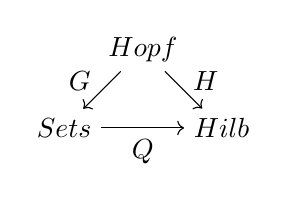
\begin{tikzpicture}
	\node (0) at (-1, 0) {$Sets$};
	\node (1) at (1, 0) {$Hilb$};
	\node (2) at (0, 1) {$Hopf$};
	\node (5) at (-0.8, 0.6) {$G$};
	\node (6) at (0.8, 0.6) {$H$};
	\node (7) at (0, -0.3) {$Q$};
	\draw [->] (2) to (0);
	\draw [->] (2) to (1);
	\draw [->] (0) to (1);
	\end{tikzpicture}
\end{center}
Clearly from the diagram we see that group algebras $\mathbb{C}G$ are hopf algebras by post-composing $G$ with $Q$. In this case the comultiplication in $Hilb$ is the linearisation of the copy map (the copy map on some basis extended linearly to the whole Hilbert space) which is co-commutative. For a general $H:Hopf \rightarrow Hilb$ this doesn't have to be the case. Hopf algebras provide a broader framework to talk about symmetry, as we can have non co-commutative Hopf algebras. Quantization of the notion of symmetry, symmetries of quantum systems. Physically we will see that Hopf algebras allow to talk about local symmetries and exchange statistics on the same footing. In particular if the Hopf algebra is not cocommutative the exchange statistics can be highly non-trivial, in which case they will describe the symmetries of anyons.\\
Recall that a group describes the symmetries of some space $X$ when it acts on it (e.g crystals, classical symmetries= symmetries of sets). If we apply the same reasoning to Hopf Algebras we have to make $H$ act on some quantum state space (i.e Hilbert space). So our object of study is not $H$ on its own but rather a module (or representation) of $H$. In the diagrammatic language we depict it as follows:
\begin{center}
	\begin{tikzpicture}[scale=0.9, black/.style={draw,regular polygon,
		regular polygon sides=4,fill=white}]
	\node (0) at (0, -1.2) {$V$};
	\node[black] (1) at (0, 0) {};
	\node (2) at (0, 1) {};
	\node (3) at (-0.7, -1.2) {$H$};
	\draw (0) to (1);
	\draw (1) to (2);
	\draw (3) to (1);
	\end{tikzpicture}
\end{center}
Where $V$ is a finite dimensional vector space. Note that the above diagram represents a process in $Vect$. All the diagrams we will be drawing from now on are about vector spaces and linear maps. In order for $V$ to be a representation the following must hold.
\begin{equation}
\begin{gathered}
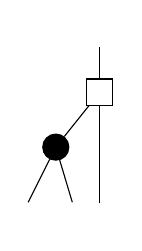
\begin{tikzpicture}[scale=0.7, squr/.style={draw,regular polygon,
	regular polygon sides=4,fill=white}, black/.style={draw,shape=circle,fill=black}]
\node (0) at (0, -2.2) {};
\node[squr] (1) at (0, 0) {};
\node (2) at (0, 1) {};
\node[black] (3) at (-0.8, -1) {};
\draw (0) to (1);
\draw (1) to (2);
\draw (3) to (1);
\draw (-1.3, -2) to (3);
\draw (-0.5, -2) to (3);
\end{tikzpicture}
\end{gathered}
\, = \,
\begin{gathered}
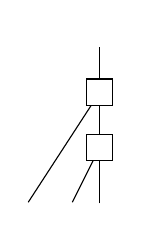
\begin{tikzpicture}[scale=0.7, squr/.style={draw,regular polygon,
	regular polygon sides=4,fill=white}, black/.style={draw,shape=circle,fill=black}]
\node (0) at (0, -2.2) {};
\node[squr] (1) at (0, 0) {};
\node (2) at (0, 1) {};
\node[squr] (3) at (0, -1) {};
\draw (0) to (3);
\draw (3) to (1);
\draw (1) to (2);
\draw (3) to (1);
\draw (-1.3, -2) to (1);
\draw (-0.5, -2) to (3);
\end{tikzpicture}
\end{gathered}
\end{equation}
Suppose $V$ and $W$ are representations of $H$, then we say $f:V \rightarrow W$ is an intertwiner if:
\begin{equation}
\begin{gathered}
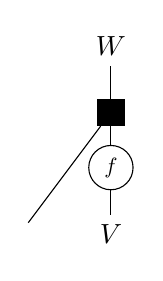
\begin{tikzpicture}[scale=0.7, squr/.style={draw,regular polygon,
	regular polygon sides=4,fill=black}]
\node (0) at (0, -2.2) {$V$};
\node[squr] (1) at (0, 0) {};
\node (2) at (0, 1.2) {$W$};
\node[scale=0.8,draw,circle] (3) at (0, -1) {$f$};
\draw (0) to (3);
\draw (3) to (1);
\draw (1) to (2);
\draw (3) to (1);
\draw (-1.5, -2) to (1);
\end{tikzpicture}	
\end{gathered}
\, = \,
\begin{gathered}
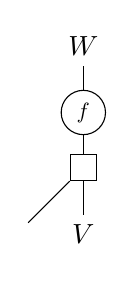
\begin{tikzpicture}[scale=0.7, squr/.style={draw,regular polygon,
	regular polygon sides=4,fill=white}]
\node (0) at (0, -2.2) {$V$};
\node[scale=0.8,draw,circle] (1) at (0, 0) {$f$};
\node (2) at (0, 1.2) {$W$};
\node[squr] (3) at (0, -1) {};
\draw (0) to (3);
\draw (3) to (1);
\draw (1) to (2);
\draw (3) to (1);
\draw (-1, -2) to (3);
\end{tikzpicture}	
\end{gathered}
\end{equation}
Where the black square denotes the action of $H$ on $W$. We obtain in this way the category of representations of $H$ denoted $Rep(H)$, where objects are $H$-modules and arrows intertwiners. This category has really nice structure induced from the properties of $H$.
$Rep(H)$ are braided fusion categories and are models for topological quantum computation, $Rep(\mathbb{C}G)$ gives Permutational quantum computing.

%%%%%%%%%%%%%%%%%%%%%%%%%%%%%%%%%%%%%%%%%%%%%%%%%%%%%%%%%%%%%%%%%%%%%%%%%%%%%%%%%%%%%%%%%%%%%%%%%%%%%%%%%%%%%%%%%%%%%%%%%%%%%%%%%%%%%%%%%%%%%%%%%%%%%%%%%%%%%%%%%%%%%%%%%%%%%%%%%%%%%%%%%%%%%%%%%%%%%%%%%%%%%%%%%%%%%%%%%%%%%%%%%%%%%%%%%%%%%%%%%%%%%%%%%%%%%%%%%%%%%%%%%%%%%%%%%%%%%%%%%%%%%%%%%%%%%%%%%%%%%%%%%%%%%%%%%%%%%%%%%%%%%%%%%%%%%%%%%%%%%%%%%%%%%%%%%%%%%%%%%%%%%%%%%%%%%%%%%%%%%%%%%%%%%%%%%%%%%%%%%%%%%%%%%%%%%%%%%%%%%%%%%%%%%%%%%%%%%%%%%%%%%%%%%%%%%%%%%%%%%%%%%%%%%%%%%%%%%%%%?%%%%%%%%%%%%%%%%%%%%%%%%%%%%%%%%%%%%%%%%%%%%%%%%%%%%%%%%%%%%%%%%%%%%%%%%%%%%%%%%%%%%%%%%%%%%%%%%%%%%%%%%%%%%%%%%%%%%%%%%%%%%%%%%%%%%%%%%%%%%%%%%%%%%%%%%%%%%%%%%%%%%%%%%%%%%%%%%%%%%%%%%%%%%%%%%%%%%%%%%%%%%%%%%%%%%%%%%%%%%%%%%%%%%%%%%%%%%%%%%

\subsubsection{Hopf Algebras and Quantum groups}
quasitriangular hopf algebras \\
\begin{definition}
Quantum double construction
\end{definition}

\subsubsection{Categories of representations}

%%%%%%%%%%%%%%%%%%%%%%%%%%%%%%%%%%%%%%%%%%%%%%%%%%%%%%%%%%%%%%%%%%%%%%%%%%%%%%%%%%%%%%%%%%%%%%%%%%%%%%%%%%%%%%%%%%%%%%%%%%%%%%%%%%%%%%%%%%%%%%%%
%%%%%%%%%%%%%%%%%%%%%%%%%%%%%%%%%%%%%%%%%%%%%%%%%%%%%%%%%%%%%%%%%%%%%%%%%%%%%%%%%%%%%%%%%%%%%%%%%%%%%%%%%%%%%%%%%%%%%%%%%%%%%%%%%%%%%%%%%%%%%%%%

\subsection{Spherical Fusion categories}

\subsubsection{Spherical categories}
\begin{definition}
monoidal categories, rigidity
\end{definition}
\begin{definition}
A pivotal category is a tensor category together with a left duality $^*$ and a monoidal natural isomorphism $\gamma:id \rightarrow -^{**}$
\end{definition}
In a pivotal category we can define traces by using the monoidal natural iso. $\gamma$.
\begin{definition}
left and right trace, left and right dimension
\end{definition}
\begin{definition}
A pivotal category is called spherical if left and right traces coincide. categorical dimension.
\end{definition}
\begin{theorem}
Rep($H$) for $H$ a hopf algebra is spherical.
\end{theorem}
\begin{proof}
With comonoid and rigid
\end{proof}


\subsubsection{Fusion categories}
\begin{definition}
The category $\mathcal{C}$ is Ab if it is enriched over abelian groups. That is all hom-sets have abelian group structures and composition of morphisms is a group homomorphism. 
\end{definition}
\begin{definition}
An Ab-category $\mathcal{C}$ is additive if it has zero object and every pair of objects has a direct sum $\oplus$.
\end{definition}
\begin{definition}
An abelian category is an additive category where every morphism has a kernel and a
cokernel and every monic (epic) is a kernel (cokernel).
\end{definition}
\begin{definition}
Let k be field, we say $\mathcal{C}$ is $k$-linear if all hom-sets are k-vector spaces and composition is bilinear.
\end{definition}
We will assume throughout the thesis that $k=\mathbb{C}$ so in particular the field is algebraically closed. 
\begin{definition}
An object $X$ in a $\mathbb{C}$-linear category is called simple if End$X=k$id$_X$.
\end{definition}
\begin{definition}
$\mathcal{C}$ is semisimple if every object is isomorphic to a direct sum of simple objects. $\mathcal{C}$ is finite if there are finitely many isomorphism classes of simple objects.
\end{definition}
\begin{definition}
A $\mathbb{C}$-linear tensor category is a fusion category if it has finite-dimensional hom-spaces, is semisimple with finitely many isomorphism classes of simple objects, the unit $\mathbf{1}$ is simple  and all objects have duals.
\end{definition}

\begin{theorem}
$Rep(H)$ is a fusion category
\end{theorem}

\begin{example}
Any group $G$ is a hopf algebra (comonoid = copy).\\
Therefore $RepG$ can also be made monoidal and rigid.
\end{example}

\begin{example}
Recall the group $S_3=\{e, g, g^2, \sigma, \sigma g, \sigma g^2 \}$. The category $Rep(S_3)$ is a fusion category. By the known representation theory of $S_3$, $Rep(S_3)$ has three simple objects: the trivial representation $1$, the sign representation $-1$ and the geometric two dimensional representation $\tau$:
\begin{equation*}
\begin{split}
    \tau : \quad & \sigma \mapsto \left( {\begin{array}{cc} 0 & 1 \\ 1 & 0 \end{array}}\right) \\
     & g \mapsto \left( {\begin{array}{cc} \omega & 0 \\ 0 & \bar{\omega} \end{array}}\right)
\end{split}
\end{equation*}
These satisfy the following fusion rules $\forall X$ simple object:
\begin{equation}
        1 \otimes X \simeq X \simeq X \otimes 1\\
        -1 \otimes -1 \simeq 1\\
        -1 \otimes \tau \simeq \tau \simeq \tau \otimes -1\\
        \tau \otimes \tau \simeq 1 \oplus -1 \oplus \tau\\
\end{equation}

\end{example}

\subsubsection{Graph invariants}
%%%%%%%%%%%%%%%%%%%%%%%%%%%%%%%%%%%%%%%%%%%%%%%%%%%%%%%%%%%%%%%%%%%%%%%%%%%%%%%%%%%%%%%%%%%%%%%%%%%%%%%%%%%%%%%%%%%%%%%%%%%%%%%%%%%%%%%%%%%%%%%%
%%%%%%%%%%%%%%%%%%%%%%%%%%%%%%%%%%%%%%%%%%%%%%%%%%%%%%%%%%%%%%%%%%%%%%%%%%%%%%%%%%%%%%%%%%%%%%%%%%%%%%%%%%%%%%%%%%%%%%%%%%%%%%%%%%%%%%%%%%%%%%%%

\subsection{Braided Fusion categories}

\subsubsection{Braiding and twisting}
Braid group, Yang-Baxter, Quasitriangular Hopf algebras. \\
\begin{definition}
Braided monoidal categories (with braid $c$)
\end{definition}
\begin{definition}
Ribbon categories (twist $\theta$)
\end{definition}
\begin{definition}
The symmetric centre $Z_2(\mathcal{C})$ of a braided tensor category $\mathcal{C}$ is the full subcategory with the following objects:
$$ \{ X \in \mathcal{C} : c_{X,Y} \circ c_{Y,X} = id_{Y\otimes X} \forall Y \in \mathcal{C} \} $$
\end{definition}

\begin{example}
Braid group $B_n$, free braid category, free construction Tensor categories $\rightarrow$ BTCs (2-adjunction)
\end{example}
\begin{example}
categories of tangles = free rigid braided categories.\\
Tangle categories are not linear over a field but can be linearised by using the free vector space functor $Set \rightarrow Vect$. This gives still big categories, but can be quotiented out by an ideal defined in terms of link-invariants to give interesting cats.
\end{example}
\begin{definition}
braided fusion category
\end{definition}
\begin{definition}
Let $\mathcal{C}$ be a tensor category, $X \in \mathcal{C}$. A half-braiding $e_X$ is a family $\{ e_X(Y):X\otimes Y \xrightarrow{\sim} Y\otimes X \}$ such that $e_X(\mathbf{1}) = id_X$ and 
\begin{equation*}
e_X(Y\otimes Z) = id_Y\otimes e_X(Z) \circ e_X(Y) \otimes id_Z \quad \forall Y,Z \in \mathcal{C}
\end{equation*}
\end{definition}

\begin{theorem}
If $\mathcal{C}$ is $k$-linear, spherical or a *-category (k-linear dagger) then so is $Z_1(\mathcal{C})$ 
\end{theorem}
\begin{theorem}
If $H$ is a quasitriangular Hopf Algebra then $Rep(H)$ is a braided fusion category.
\end{theorem}

N-matrix, R-matrix


\subsubsection{Modular categories}

\begin{definition}
The symmetric center $Z_2(\mathcal{C})$ is the full subcategory of $\mathcal{C}$ defined by:
$$ obj \, Z_2(\mathcal{C}) = \{ X\in \mathcal{C} : c_{X,Y} \circ c_{Y,X} = id_{Y\otimes X} \quad \forall Y \in \mathcal{C} \} $$
\end{definition}
\begin{definition}
A braided fusion category is:
\begin{itemize}
    \item pre-modular if it is spherical,
    \item non-degenerate if $Z_2(\mathcal{C})$ is trivial
    \item modular if it is pre-modular and non-degenerate.
\end{itemize}
\end{definition}

\begin{theorem}
Let $\mathcal{C}$ be a spherical symmetric fusion category with trivial twists. Then $\mathcal{C} \simeq Rep(G)$ for some group $G$ (unique up to iso).
\end{theorem}

\begin{theorem}
If $\mathcal{C}$ is a spherical fusion category then $Z_1(\mathcal{C})$ is modular.
\end{theorem}
Modular tensor categories are particularly well behaved types of braided fusion categories. To any modular category $\mathcal{C}$ we can assign the so called modular $S$-matrix which will contain all the information of the fusion rules as well as the braided structure.
\begin{definition}
Let $\mathcal{C}$ be a spherical braided fusion category and let $I$ be the set of isomorphism classes of simple objects in $\mathcal{C}$. We define $S_{i,j}$ for $i,j \in I$ to be the following: (diagram)
\end{definition}
\begin{theorem}
$\mathcal{C}$ is modular iff the $S$-matrix is invertible.
\end{theorem}
\begin{theorem}
The modular $S$-matrix diagonalises the $N$-matrix.
\end{theorem}
splitting, fusion rules, braided, R,T matrices, modular S matrix.

\subsubsection{Knot invariants}

%%%%%%%%%%%%%%%%%%%%%%%%%%%%%%%%%%%%%%%%%%%%%%%%%%%%%%%%%%%%%%%%%%%%%%%%%%%%%%%%%%%%%%%%%%%%%%%%%%%%%%%%%%%%%%%%%%%%%%%%%%%%%%%%%%%%%%%%%%%%%%%%
%%%%%%%%%%%%%%%%%%%%%%%%%%%%%%%%%%%%%%%%%%%%%%%%%%%%%%%%%%%%%%%%%%%%%%%%%%%%%%%%%%%%%%%%%%%%%%%%%%%%%%%%%%%%%%%%%%%%%%%%%%%%%%%%%%%%%%%%%%%%%%%%
%%%%%%%%%%%%%%%%%%%%%%%%%%%%%%%%%%%%%%%%%%%%%%%%%%%%%%%%%%%%%%%%%%%%%%%%%%%%%%%%%%%%%%%%%%%%%%%%%%%%%%%%%%%%%%%%%%%%%%%%%%%%%%%%%%%%%%%%%%%%%%%%
%%%%%%%%%%%%%%%%%%%%%%%%%%%%%%%%%%%%%%%%%%%%%%%%%%%%%%%%%%%%%%%%%%%%%%%%%%%%%%%%%%%%%%%%%%%%%%%%%%%%%%%%%%%%%%%%%%%%%%%%%%%%%%%%%%%%%%%%%%%%%%%%

\section{The Physics of Anyons}

%%%%%%%%%%%%%%%%%%%%%%%%%%%%%%%%%%%%%%%%%%%%%%%%%%%%%%%%%%%%%%%%%%%%%%%%%%%%%%%%%%%%%%%%%%%%%%%%%%%%%%%%%%%%%%%%%%%%%%%%%%%%%%%%%%%%%%%%%%%%%%%%
%%%%%%%%%%%%%%%%%%%%%%%%%%%%%%%%%%%%%%%%%%%%%%%%%%%%%%%%%%%%%%%%%%%%%%%%%%%%%%%%%%%%%%%%%%%%%%%%%%%%%%%%%%%%%%%%%%%%%%%%%%%%%%%%%%%%%%%%%%%%%%%%

\subsection{Phases of Matter}
Classical phases of matter: solid, liquid and gas.\\
Temperature is proportional to energy \\
Close to zero temperature, phases of matter are quantized. We obtain exotic behaviours of matter.\\
In order to talk about quantum phases of matter we need to consider many-body quantum systems. We will use the definitions of Zhenghan

\subsubsection{Many-body Quantum Systems}
\begin{definition}
A Many-body Quantum system (MQS), is a triple $(\mathcal{L}, b, \mathcal{H})$, where $\mathcal{L}$ is a Hilbert space with a distinguished ONB $b$ and a hermitian operator $\mathcal{H}: \mathcal{L} \rightarrow \mathcal{L}$, called Hamiltonian.
\end{definition}
The eigenvalues of the Hamiltonian correspond to the energy levels of the system. The elements of the basis $b$ are the initial classical states of the system. Many-body quantum systems will usually be obtained from spatial configurations of particles, which we will descibe by graphs.
\begin{definition}
A Hamiltonian is k-local if...
\end{definition}

\begin{definition}
An MQS on a graph $\Tau = (V,E)$ with $\mathbb{C}^d$ degrees of freedom (qudit space) is an MQS $(\mathcal{L},b, \mathcal{H})$ where
$$ \mathcal{L} = \otimes_{e\in E} \mathbb{C}^d$$
$b$ is obtained from the standard basis of $\mathbb{C}^d$ and $\mathcal{H}$ is a local Hamiltonian.
\end{definition}
Many interesting spatial configurations of matter are obtained from triangulations of manifolds by taking their 1-skeleton graph.\\
Let us consider unitary operators which commute with the Hamiltonian $\mathcal{H}$. These are operators which leave the energy of the system unchanged. These transformations form a group $G$ under composition and a particle subject to the Hamiltonian $\mathcal{H}$ will be described by irreducible representations of $G$. $G$ is the group of symmetries of the system under $\mathcal{H}$.

\begin{proposition}
Let $\mathcal{H}:V\rightarrow V$ be the Hamiltonian for some physical system described by a hilbert space $V$. Then the unitary operators which commute with $\mathcal{H}$ form a group $G$.
\end{proposition}
\begin{proof}
Suppose $R_1\ham=\ham R_1$ and $R_2\ham=\ham R_2$, then $R_1R_2\ham=R_1\ham R_2 = \ham R_1R_2$. Also $R^{-1}\ham = R^{-1}\ham RR^{-1} = R^{-1}R\ham R^{-1} =\ham R^{-1}$. The unit is the identity operator $id_{V^*\otimes V}$.
\end{proof}

\begin{proposition}
If $G$ is the group of symmetries of a Hamiltonian $\mathcal{H}$ then each energy eigenspace carries an irreducible representation of $G$.
\end{proposition}
\begin{proof}
Note that under the obvious $G$-action, $V$ is a representation of $G$. 
The eigenvalues of the Hamiltonian, correspond to energy levels of the physical system which we previously called 'particle types'. Fix any eigenvalue $E$ of $\ham$, the allowed states of a particle with energy $E$ live in the corresponding eigenspace $V_E$. Indeed these are invariant under the action of $\ham$:
$$ \ham \ket{\psi}= E\ket{\psi}$$
Note that if $R\in G$ then
$$ \ham R \ket{\psi}=R\ham \ket{\psi}=ER\ket{\psi}$$
So $R\ket{\psi}$ is an eigenvector with eigenvalue $E$. Therefore $G$ acts on $V_E$ for any energy level.
We prove $V_E$ is irreducible by showing that $End(V_E) \simeq \mathbb{C}$. Indeed suppose $f:V_E \rightarrow V_E$ is an intertwiner, then $fR=Rf \, \forall R \in G$
TO PROVE
\end{proof}
Starting with a hamiltonian $\ham$ we have shown that energy levels (or particle types) correspond to the irreducible representations of the group $G$ of symmetries of $\ham$. The particle theory correponding to the hamiltonian $\ham$ has irreducible representations of $G$ as objects and intertwiners, preserving the energy of the system, as processes. This is the definition of the category $Rep(G)$. Note there are no restrictions yet on the group of symmetries.
\begin{example}
Suppose $\ham = \sigma_Z$ be the Hamiltonian of a qubit living in $\mathbb{C}^2$. It has eigenvalues $\pm1$ and corresponding eigenvectors $\ket{0}$ and $\ket{1}$.. The group algebra of symmetries of $\ham$ is generated by $id$ and $\ham$ and it is isomorphic to $\mathbb{C}\mathbb{Z}_2$. $\mathbb{Z}_2$ has two irreducible representations (the trivial and the sign) representations which correspond to the one-dimensional eigenspaces of $\ham$. Note that 
\end{example}

\subsubsection{Topological phases of matter}
Let us consider $N$ indistinguishable particles evolving in space. The quantum amplitude for a space-time evolution of the system will depend on the topology of the particle word-lines and not on the detailed geometry. \\
example: particle-antiparticle creation, swap and annihilation\\
To formalize the situation suppose we have $N$ indistinguishable particles in $D$ dimensions, the configuration space can be written as:
$$ \mathrm{C}=(\mathbb{R}^{ND}-\Delta)/S_N$$
Where $\Delta$ is the space of coincidences where at least two of the $N$ particles occupy the same position in $\mathbb{R}^D$. We are quotienting the space by $S_N$ to account for the indistinguishability of the particles (i.e we do not care about the order of the $N$ coordinates in $D$ dimensions). The space of paths through confuguration space $\mathrm{C}$ divides into topologically distinct classes, described by the fundamental group $\pi_1(\mathrm{C})$.\\
If we fix the starting and endpoint in the configuration space, we can describe the evolution of the wave function for the system  via unitary transformations induced from the element of the fundamental group corresponding to particles word-lines. In mathematical terms this corresponds to a representation of the group of homotopy classes of paths from starting to endpoint on the configuration space. \\
If space-time has $D=3+1$ dimensions,  the topological class of paths is completely determined by the corresponding permutation of the particles, because there are no knots in $4$ dimensions. Therefore the evolution of the system will be described by a representation of the symmetric group $S_N$. \\
In $2+1$ dimensions we have more exotic behaviour, as the paths in configuration space can braid. The time evolution of the wave function is then described by a representation of the braid group on $N$ strands, denoted $B_N$.

\begin{itemize}
    \item Abelian case
\end{itemize}
We say the system is abelian if the wave function lives in a one-dimensional representation of the group of paths in configuration space. IN $3+1$ dimensions, this means we have to consider the one-dimensional representations of $S_N$. Note that there are only two possibilities (namely the trivial and the sign representations) corresponding to the two possible types of particle statistics in $3+1$ dimensions (Bose and Fermi statistics respectively). \\
In $2+1$ dimensions we have many more possibilities as the evolution of the wave function will be described by a one-dimensional representation of the braid group $B_N$. There are infinitely many one dimensional representations of the braid group connecting the fermions and bosons case. These are described by a single parameter $\theta$. Only one parameter because using Yang-Baxter we can show that all $N$ phases have to be the same, also can show $\theta$ has to be a fraction from physical considerations. We obtain abelian anyons. \\
\begin{itemize}
    \item Non-abelian case
\end{itemize}
In $3+1$ dimensions we don't get anything more than bosons and fermions if we also want to consider creation, annihilation (splitting, fusion) of particles (Doplicher-Roberts theorem).\\
In $2+1$ dimensions we obtain degeneracy, non-abelian anyons, braidings give all unitaries.\\~\\
In the previous section, we only considered groups of symmetries of a Hamiltonian. In order take topological symmetries of a system into account, we need the more general framework of Hopf Algebras. In particular, as those symmetries arise from braids, we need quasitriangular hopf algebras (or quantum groups) to treat all symmetries on the same level. We will see taht the universal $R$-matrix plays an important role in the description of topological dependencies.\\

%%%%%%%%%%%%%%%%%%%%%%%%%%%%%%%%%%%%%%%%%%%%%%%%%%%%%%%%%%%%%%%%%%%%%%%%%%%%%%%%%%%%%%%%%%%%%%%%%%%%%%%%%%%%%%%%%%%%%%%%%%%%%%%%%%%%%%%%%%%%%%%%
%%%%%%%%%%%%%%%%%%%%%%%%%%%%%%%%%%%%%%%%%%%%%%%%%%%%%%%%%%%%%%%%%%%%%%%%%%%%%%%%%%%%%%%%%%%%%%%%%%%%%%%%%%%%%%%%%%%%%%%%%%%%%%%%%%%%%%%%%%%%%%%%

\subsection{Algebraic theory of Anyons}
In this section we describe the algebraic framework of modular categories, as theories of anyons. \\
Let us first set some labels $a,b,c...$ for our particle types. Let us label by $\mathbf{1}$ the vacuum particle type "no-particle". It has the property that it leaves other particle types unchanged under fusion: $1 \otimes a \simeq a \simeq a \otimes 1$. So for the moment our theory is a monoidal category $\mathcal{C}$ and we can already use the diagrammatic language, the wires carry particle types (image). Now note that fusion $a \otimes b \xrightarrow{\sim} c$ and splitting $c \xrightarrow{\sim} a \otimes b$ are really dual concepts. This duality is witnessed by the existence of antiparticles. Each particle $a$ comes with its antiparticle $a^*$ such that $a\otimes a^* \simeq 1 \simeq a^* \otimes a$. So the category must be rigid, we will assume it is a well behaved category i.e it is spherical and $1^*=1$. So we can define the quantum numbers for each particle type (image). At this point we need to linearise the theory to take superpositions into account. We enrich the category over commutative monoids and introduce a biproduct $\oplus$ and zero object $\mathbf{0}$ as additional structure on $\mathcal{C}$. In order for the fusion to behave well with superpositions we must require that our particle types be simple objects in the category. At this point, our category $\mathcal{C}$ is a spherical fusion category and the fusion rules look like this:
\begin{equation}
a\otimes b \simeq \oplus_c N_{ab}^c c
\end{equation}
Where $N_{ab}^c \in \mathbb{N}$. \\
We still have one question to ask to the theory, what happens when a particle is passed around another one? To answer this question the theory must have a braid structure and we obtain a braided fusion category (see section 1).
The braid structure determines the long-distance, topological interactions between particles. We can place braided fusion categories in a spectrum by asking what their symmetric center $Z_2$ is. The two antipodal points of this spectrum are symmetric fusion categories on one side (such that $Z_2(\mathcal{C})=\mathcal{C}$) and modular tensor categories (such that the symmetric centre is trivial, i.e its objects are direct products of the tensor unit $\mathbf{1}$). In the first case, we have only symmetric exchange symmetries so that all particles in the theory are either bosons or fermions. Such categories are degenerate anyon theories with no topological dependencies between particles. Modular tensor categories are really the opposite situation, the theory doesn't contain any bosons or fermions but only non-degenerate anyons, i.e anyons with non-trivial twist factor.

\begin{example}
Suppose we start from a set of labels and define the fusions to form a group. In fact $1$ is the identity particle type, for any particle type $a$, $a^*$ will be its inverse. We have defined the skeleton of a spherical fusion category, which we obtain by linearising, i.e taking a functor to $Hilb$. We obtain the category $RepG$, in which the allowed linear processes (intertwiners) preserve the fusion rules. Doing the process and then fusing the system with a particle (action of the group) is the same as doing the fusion and then the process. 
The category $Rep(G)$ for $G$ a group is a spherical fusion category. Linearity and tensor are given by the underlying $Vect$ structure, simple objects are the irreducible representations of $G$, duality is proved by using the group inverse (hopf algebra antipode). For $G=\mathbb{Z}_2$ we have two irreducible representations $\tau_+$ and $\tau_-$, both one dimensional with the obvious fusion rules given by the cyclic group of order $2$.\\
Let us consider the object $V=\mathbb{C}G$ of $RepG$. (Note $V \simeq \oplus_i V_i$ where $V_i$'s are the simple objects.) Simple objects correspond to particle types so the states of $V$ are superpositions of particle types. In the case where $G$ is abelian there is only one way two particles can fuse to a third, so the fusions are deterministic and the irreducible representations will be one dimensional, each corresponding to an element of the group. If $G$ is not abelian, say $a\otimes b \simeq c_1$ and $b \otimes a \simeq c_2$ then taking the representations category defines a 2-dimensional object $c$ spanned by $\{c_1,c_2\}$ which is an irreducible representation of $G$. So from now on we will call particle types the irreducible representations and particles subtypes the elements of the group $G$.  The action of $G$ permutes the basis vectors, multiplying by an element of $G$, but an element of $G$ is precisely a particle subtype and multiplication is fusion. So acting with $g \in G$ on a state $v \in V$ corresponds to fusing a particle of type $g$ with one that is in a superposition $v$ of particle types. The allowed processes are intertwiners which commute with the action and therefore preserve fusions. If the group $G$ is abelian, then the particles are abelian anyons.
\end{example}

\begin{theorem}
RepG is a braided fusion category
\end{theorem}

%%%%%%%%%%%%%%%%%%%%%%%%%%%%%%%%%%%%%%%%%%%%%%%%%%%%%%%%%%%%%%%%%%%%%%%%%%%%%%%%%%%%%%%%%%%%%%%%%%%%%%%%%%%%%%%%%%%%%%%%%%%%%%%%%%%%%%%%%%%%%%%%
%%%%%%%%%%%%%%%%%%%%%%%%%%%%%%%%%%%%%%%%%%%%%%%%%%%%%%%%%%%%%%%%%%%%%%%%%%%%%%%%%%%%%%%%%%%%%%%%%%%%%%%%%%%%%%%%%%%%%%%%%%%%%%%%%%%%%%%%%%%%%%%%

\subsection{Quantum Symmetry}
Recall our discussion from the subsection Algebraic theory of anyons. We distinguished degenerate anyons theories (symmetric fusion categories) to modular tensor categories. In this section we will look at physically implementable examples of those two cases, and discuss a general construction for taking a degenerate anyon theory and making it modular.\\
Local symmetries are very well described by the theory of groups. In order to describe symmetries of Hamiltonians exhibiting topological phases of matter we need to use the more general notion of Hopf Symmetry.

\subsubsection{The Quantum Double}
Let us consider a two dimensional lattice of particles (situated on the edges of the lattice) under the influence of a magnetic field and an electric field. Anyonic behaviour is exhibited by excitations of the particles on the lattice. In our process theory the allowed processes are charge-flux composites, the states are lattice configurations (determined by the states of the particles, which are generally given by an element $g \in G$)  . By mearuring the flux in certain regions of the lattice and acting on the charge of the corresponding flux sector we can create and control the behaviour of excitations on the material.
\begin{example}
Let us consider the case where $G \simeq \mathbb{Z}_2$. We obtain a lattice of spins. Those particles we wont use as our qubits, indeed we will impose that their state is in a basis state $\{\ket{0},\ket{1}\}$. One way to picture the states of the system is to draw the lattice and colour the edges red when the corresponding particle is in state $\ket{0}$. Note that the lattice can be embedded in any manifold (e.g. subsection quantum memory is a lattice on a torus, if we used a more layered lattice we could implement error correction). What we obtain is a picture of paths on the lattice which we call excitations.
\end{example}
The magnetic flux of a particle is given by an element $h \in G$, this indexes the superselection sectors so that the charge lives in a unitary irreducible representation of the centralizer $N(h)$ of the flux $h$ carried by the particle. We have two possible operations on our states: flux measurement and symmetry transformations on the charge. Flux measurements correspond to a projection $P_h \in \mathbb{C}G^*$ onto flux sector $h$. The residual global symmetry transformations are then implemented via some $g \in N(h)$. \\
Naturally the projectors form a Von Neumann family and satisfy 
$$P_hP_{h'}= \delta_{h,h'} P_h.$$ 
A general element $g \in G$ is a global symmetry transformation and affects the fluxes via conjugation:
\begin{equation}
gP_h = P_{ghg^{-1}}g
\end{equation}
The quantum double construction allows to capture both global symmetry transformations and projective measurements in one algebraic structure.
\begin{definition}
Lagrangian, Noether's theorem
\end{definition}
\begin{definition}
For any finite group $G$, its quantum double $D(G)$ is the algebra generated by $\{P_hg\}_{h,g\in G}$ with multiplication induced by (1). $D(G) \simeq \mathbb{C}G^* \otimes \mathbb{C}G$ and inherits their hopf algebra structure (comultiplication and antipode are given by tensoring). 
\end{definition}
$D(G)$ has a natural quasi-triangular structure witnessed by the universal R-matrix $R=\sum_{g,h \in G}P_he \otimes P_hg$, making $RepDG$ braided. Particle states then live in irreducible representations of $D(G)$. Let $\{C_i\}_{i=1}^n$ be the distinct conjugacy classes in $G$. To each of those conjugacy classes corresponds a centralizer subgroup $N_i$ (two choices of representatives for $C_i$ yield isomorphic centralizer subgroups). Then for any irreducible representation $(\alpha,V^i_\alpha)$ of $N_i$ with basis elements $v^\alpha_j$, let $V_{i,\alpha} = \mathbb{C}C_i \otimes V^i_\alpha$, this has basis $\{ \ket{k,v^\alpha_j} \}_{j=1,...,dim\alpha}^{k\in C_i}$ and forms an irreducible representation of $D(G)$ under the action 
\begin{equation}
P_hg\ket{k,v^\alpha_j} = \delta_{h,gkg^{-1}} \ket{h,\alpha(h^{-1}gk)v^\alpha_j}
\end{equation}
and the $\{V_{i,\alpha}\}$ is the complete set of irreducible representations.


\subsubsection{Drinfeld center}
\begin{definition}
The braided (Drinfeld) centre of $\mathcal{C}$ is the category $Z_1(\mathcal{C})$ with objects pairs $(X,e_X)$ where $X \in \mathcal{C}$ and $e_X$ is a half-braiding, and with morphisms given by the morphisms of $\mathcal{C}$ which commute with the half-braiding.
\end{definition}
\begin{theorem}
$Z(RepG) \simeq RepDG$
\end{theorem}
\subsubsection{Kitaev's lattice construction}
The following argument seems to work for abelian groups.
Being a spherical fusion category, $RepG$ is well suited to be a process theory of particles. As we pointed out earlier what is missing is the braided structure, but let us ignore this for the moment. We have simple objects corresponding to particle types and fusion rules determined by the group structure.\\
Now suppose we have particles whose fusion is described by a $RepG$ and let us consider a lattice with those particles located at the edges. This lattice could be embedded in any space but let us assume it is a lattice on a torus. The states of our system are then configurations of particle types on the edges. So edges are coloured by simple representations from $RepG$. Now we can act on the lattice with vertex and plaquette operators which basically implement measurements at vertices and flips (fusion with other simple reps) of the particles on a plaquette. By now we have produced a theory where states are lattice configurations and processes are generated by vertex $V_\alpha$ and plaquette $P_\beta$ operators. We want to extract the topological degrees of freedom of this theory. First we note that using vertex operators we can make sure that the product of all particles incident at all vertices is 1, i.e $V_\alpha=1$ $\forall \alpha$. We restrict our states to satisfy this local property and we drop vertex operators (in the sense that they are not allowed processes anymore), indeed we fixed their value at all points of the lattice. By also setting $P_\beta =1$ at all plaquettes we quotient further the theory. So we obtain a theory where all vertex and plaquette measurements have value $1$. We finally declare two configurations to be equal if there is a sequence of plaquette operations taking us from one to the other. Noting that plaquette operators are local isometries we see this corresponds to quotienting out the category by an equivalence relation. This doesn't exaust the degrees of freedom of the theory because of the topology of the torus. Those topological degrees of freedom will be the simple objects our newly created category, their fusion rules are completely determined by the structure of $Rep(G)$. Indeed the category we obtained is $Z(Rep(G)) \simeq Rep(DG)$.

\begin{theorem}
The lattice construction and the Drinfeld construction coincide
\end{theorem}

\begin{example}
In the case $G=\mathbb{Z}_2$, recall $Rep\mathbb{Z}_2$ has two simple object of dimension one $\tau_+$ and $\tau_-$ with fusions given by group structure. Let us draw the states of our system as colourings of the edges of the lattice. The condition on the vertex operators results in no endlines and no triple intersections on the lattice. The condition on plaquette operators only allows loop configurations. Quotienting out by plaquette operators relation we obtain 4 distinct classes, namely the vacuum $1$, the first cycle of the torus $X$, the second cycle $Z$, and both cycles $X \otimes Z \simeq Y$ and we have the fusion rules. The theory we have obtained is $RepD\mathbb{Z}_2$ which has in fact 4 simple objects with same fusions. We are therefore treating the topological defects of a theory in $Rep\mathbb{Z}_2$ as particles particles in their own right, with their own theory. All those representations are one-dimensional and in fact we just formulated a theory of abelian anyons.
\end{example}

%%%%%%%%%%%%%%%%%%%%%%%%%%%%%%%%%%%%%%%%%%%%%%%%%%%%%%%%%%%%%%%%%%%%%%%%%%%%%%%%%%%%%%%%%%%%%%%%%%%%%%%%%%%%%%%%%%%%%%%%%%%%%%%%%%%%%%%%%%%%%%%%
%%%%%%%%%%%%%%%%%%%%%%%%%%%%%%%%%%%%%%%%%%%%%%%%%%%%%%%%%%%%%%%%%%%%%%%%%%%%%%%%%%%%%%%%%%%%%%%%%%%%%%%%%%%%%%%%%%%%%%%%%%%%%%%%%%%%%%%%%%%%%%%%
%%%%%%%%%%%%%%%%%%%%%%%%%%%%%%%%%%%%%%%%%%%%%%%%%%%%%%%%%%%%%%%%%%%%%%%%%%%%%%%%%%%%%%%%%%%%%%%%%%%%%%%%%%%%%%%%%%%%%%%%%%%%%%%%%%%%%%%%%%%%%%%%
%%%%%%%%%%%%%%%%%%%%%%%%%%%%%%%%%%%%%%%%%%%%%%%%%%%%%%%%%%%%%%%%%%%%%%%%%%%%%%%%%%%%%%%%%%%%%%%%%%%%%%%%%%%%%%%%%%%%%%%%%%%%%%%%%%%%%%%%%%%%%%%%


\section{Quantum Computation}

%%%%%%%%%%%%%%%%%%%%%%%%%%%%%%%%%%%%%%%%%%%%%%%%%%%%%%%%%%%%%%%%%%%%%%%%%%%%%%%%%%%%%%%%%%%%%%%%%%%%%%%%%%%%%%%%%%%%%%%%%%%%%%%%%%%%%%%%%%%%%%%%
%%%%%%%%%%%%%%%%%%%%%%%%%%%%%%%%%%%%%%%%%%%%%%%%%%%%%%%%%%%%%%%%%%%%%%%%%%%%%%%%%%%%%%%%%%%%%%%%%%%%%%%%%%%%%%%%%%%%%%%%%%%%%%%%%%%%%%%%%%%%%%%%

\subsection{Permutational Quantum Computing}
\subsubsection{Jordan's model}
Here we give a categorical description of Jordan's model for Permutational Quantum computation [REFERENCE].

\begin{definition}
Let $\mathcal{J}$ be the symmetric fusion category with positive half integers as simple objects, fusions etc.
\end{definition}

\subsubsection{Categorical PQC}
The construction given by Jordan can be generalised. In this section we argue that Symmetric Fusion categories are models fo permutational quantum computation.

\begin{theorem}
Any symmetric fusion category induces representations of the symmetric group $S_n$ for any $n\in \mathbb{N}$.
\end{theorem}

\begin{theorem}
If $\mathcal{C}$ is a symmetric fusion categories, then $\mathcal{C}$ is symmetrically monoidally equivalent to $Rep(G)$ for $G$ some group (if the twist is trivial) or some supergroup (if the twist is -1).
\end{theorem}
\begin{proof}
Doplicher-Roberts theorem
\end{proof}

\begin{proposition}
Jordan's model $\mathcal{J}$
\end{proposition}
\begin{example}
Permutational quantum computation in $Rep(S_3)$.
\end{example}

\subsubsection{Spin Network Quantum systems}
The model described by Jordan is implementable by defining a hamiltonian on a network of spins.\\
Generalised spin network systems for arbitrairy group $G$


%%%%%%%%%%%%%%%%%%%%%%%%%%%%%%%%%%%%%%%%%%%%%%%%%%%%%%%%%%%%%%%%%%%%%%%%%%%%%%%%%%%%%%%%%%%%%%%%%%%%%%%%%%%%%%%%%%%%%%%%%%%%%%%%%%%%%%%%%%%%%%%%
%%%%%%%%%%%%%%%%%%%%%%%%%%%%%%%%%%%%%%%%%%%%%%%%%%%%%%%%%%%%%%%%%%%%%%%%%%%%%%%%%%%%%%%%%%%%%%%%%%%%%%%%%%%%%%%%%%%%%%%%%%%%%%%%%%%%%%%%%%%%%%%%

\subsection{Topological Quantum Computation}
\subsubsection{The Toplogical Model}
Hard to actually get qubits\\
Take the fusion space to be our topological hilbert space.\\
Topological qudits are usually encoded as fusion tree basis elements\\
Topologial gates: braids (can express as action of the braid group) + measurements (=fusions and associators).


\subsubsection{Anyon Vacuum on a Torus and Quantum Memory}
If we consider the torus as our configuration space. Let $C_1$, $C_2$ be the two cycles. Consider the process $T_i$ for $i=1,2$ which creates a particle-antiparticle pair, moves them in opposite directions around cycle $C_i$ so that they meet on the other side of the torus and annihilate. Then we can show $T_i$ do not commute with each other if the particles are abelian anyons with $\theta \neq 0, \pi$. We know $\theta$ must be a fraction $p/q$ with $p$ and $q$ coprime. Then we can show that the system has degenerate ground states. We have $q$ different ground state, so the vacuum state lives in a $q$ dimensional space. If we initialise it in some superposition it will remain in that state unless a $T_1$ or $T_2$ operation is implemented. Because of their topological nature it is very unlikely that such processes occur spontaneously, and therefore the quantum information stored in the superposition is protected.

\subsubsection{Approximation of Dijkgraaf-Witten link invariants}
The link invariant essentially counts homomorphisms from the fundamental group
of the link complement to the group G. (cite Zhenghan?)

%%%%%%%%%%%%%%%%%%%%%%%%%%%%%%%%%%%%%%%%%%%%%%%%%%%%%%%%%%%%%%%%%%%%%%%%%%%%%%%%%%%%%%%%%%%%%%%%%%%%%%%%%%%%%%%%%%%%%%%%%%%%%%%%%%%%%%%%%%%%%%%%
%%%%%%%%%%%%%%%%%%%%%%%%%%%%%%%%%%%%%%%%%%%%%%%%%%%%%%%%%%%%%%%%%%%%%%%%%%%%%%%%%%%%%%%%%%%%%%%%%%%%%%%%%%%%%%%%%%%%%%%%%%%%%%%%%%%%%%%%%%%%%%%%
%%%%%%%%%%%%%%%%%%%%%%%%%%%%%%%%%%%%%%%%%%%%%%%%%%%%%%%%%%%%%%%%%%%%%%%%%%%%%%%%%%%%%%%%%%%%%%%%%%%%%%%%%%%%%%%%%%%%%%%%%%%%%%%%%%%%%%%%%%%%%%%%
%%%%%%%%%%%%%%%%%%%%%%%%%%%%%%%%%%%%%%%%%%%%%%%%%%%%%%%%%%%%%%%%%%%%%%%%%%%%%%%%%%%%%%%%%%%%%%%%%%%%%%%%%%%%%%%%%%%%%%%%%%%%%%%%%%%%%%%%%%%%%%%%


\section{A braided programming language}

%%%%%%%%%%%%%%%%%%%%%%%%%%%%%%%%%%%%%%%%%%%%%%%%%%%%%%%%%%%%%%%%%%%%%%%%%%%%%%%%%%%%%%%%%%%%%%%%%%%%%%%%%%%%%%%%%%%%%%%%%%%%%%%%%%%%%%%%%%%%%%%%
%%%%%%%%%%%%%%%%%%%%%%%%%%%%%%%%%%%%%%%%%%%%%%%%%%%%%%%%%%%%%%%%%%%%%%%%%%%%%%%%%%%%%%%%%%%%%%%%%%%%%%%%%%%%%%%%%%%%%%%%%%%%%%%%%%%%%%%%%%%%%%%%

\subsection{Non-commutative linear logic}


%%%%%%%%%%%%%%%%%%%%%%%%%%%%%%%%%%%%%%%%%%%%%%%%%%%%%%%%%%%%%%%%%%%%%%%%%%%%%%%%%%%%%%%%%%%%%%%%%%%%%%%%%%%%%%%%%%%%%%%%%%%%%%%%%%%%%%%%%%%%%%%%
%%%%%%%%%%%%%%%%%%%%%%%%%%%%%%%%%%%%%%%%%%%%%%%%%%%%%%%%%%%%%%%%%%%%%%%%%%%%%%%%%%%%%%%%%%%%%%%%%%%%%%%%%%%%%%%%%%%%%%%%%%%%%%%%%%%%%%%%%%%%%%%%

\subsection{Adjunction}
This section is dedicated to the relationship between a category $\mathcal{C}$ and its braided centre $Z(\mathcal{C})$. In the first part we will talk about non-commutative logic and modalities. In the second part we will see \\

Free forgetful adjunction:
$$\Box: \mathcal{C} \rightleftarrows Z(\mathcal{C}):U$$ \\


$$\Box: RepG \rightarrow RepDG\simeq Z(RepG)$$
\begin{theorem}
Let $\{X_i\}_{i\in I}$ be the set of representatives of the isomorphism classes of simple objects in $RepG$. Let $\mathbb{C}G$ be the regular representation, then $$\mathbb{C}G \simeq \oplus_{i\in I}X_i\otimes X_i^*$$
\end{theorem}
\begin{theorem}
$\Box V = \oplus_{i\in I}X_i^*\otimes V \otimes X_i$ with action of $DG$ given by ....
\end{theorem}
Let $G$ be a group, $DG$ its quantum double, $(\pi,V)$ a representation of $G$. \\
The induced representation $\Box V$ is the coequalizer of: \\
$$DG \otimes \mathbb{C}G \otimes V \rightrightarrows DG\otimes V$$ 
Where the top arrow is given by the right action of $G$ on $DG \simeq \mathbb{C}G^* \otimes \mathbb{C}G$ 
$$ (P_hg, k) \mapsto P_h (gk^{-1})$$
(this satisfies the axioms of an action but do we have to make the action conjugate the flux projection component?) and the bottom arrow is given by the $\pi$ action on $V$. \\
To compute the coequalizer we consider the orbits of the action of $G$ on $DG$, these form a partition of $DG$:
$$ \{[P_ke] : k \in G\} $$
So, as a vector space $\Box V \simeq \mathbb{C}G \otimes V$ and the action of $DG$ on $\Box V$ is given by:
\begin{equation}
P_hg [P_ke]v = \delta_{h,gkg{-1}} [P_he] \pi(g)v
\end{equation} 
So that element $P_hg$ implements residual symmetry $g$ and projects onto flux sector $gkg^{-1}$. \\
Note that if $C_i$ are the conjugacy classes of $G$ then $\mathbb{C}G \simeq \oplus_i \mathbb{C}C_i$ and we could try to decompose:
\begin{equation}
\Box V \simeq \oplus_i \mathbb{C}C_i \otimes V
\end{equation}
The action (3) factors through the conjugacy classes, (4) gives us a decomposition of $ \Box V$ into irreducibles if $V$ is simple in $RepG$? (this hold for abelian groups, should be generalised given decomposition of $V$ into $Z_i$ modules). \\
$\Box$ is clearly not monoidal if we take $\otimes$ as tensor, is it monoidal under $\oplus$? i.e is it additive? (Note that the induced representation functor $Ind_H^G$ for $H$ subgroup of $G$ is additive). If it is additive then it is left and right exact and could use this to find the decomposition of $ \Box V$ \\
Is the $\Box$ functor representable? In the sense $\Box \simeq Hom(\mathbb{C}G,\_)$?


\begin{example}
If $G=\mathbb{Z}_2= \{e,a\}$, irreducible representations are the trivial $\tau_+$ and the one dimensional sign representation $\tau_-$. $DG \simeq \mathbb{C}\mathbb{Z}_2^* \otimes \mathbb{C}\mathbb{Z}_2$ and the orbits of the right action of $\mathbb{Z}_2$ on $D\mathbb{Z}_2$ are given by
$$ \{ [P_ee], [P_ae] \}$$
Recall that $D\mathbb{Z}_2$ has 4 irreducible one dimensional representations which we denoted $1$,$X$,$Z$,$Y$. With fusion rules generated by $A \otimes A \simeq 1$ and $X \otimes Y \simeq Z$. \\
Now let us calculate $\Box \tau_-$, it has basis $\{[P_ee] =:w_e, [P_ae] =:w_a \}$ and 
\begin{equation*}
P_ee(xw_e + yw_a)= xw_e \\
P_ae(xw_e + yw_a)= yw_a \\
P_ea(xw_e + yw_a)= -xw_e \\ 
P_aa(xw_e + yw_a)= -yw_a
\end{equation*}
And we see from the table (see Lahtinen "The Toric Code and the Quantum Double" for table of reps) that $\Box \tau_- \simeq X \oplus Y$. Similarly $\Box \tau_+ \simeq 1 \oplus Z$. \\
Consider the regular representation $V := \mathbb{C}\mathbb{Z}_2 \simeq \tau_+ \oplus \tau_-$, then $\Box V \simeq 1 \oplus X \oplus Z \oplus Y \simeq (1 \oplus X) \otimes (1 \oplus Z) $.\\
What happens if we braid the two components of $\Box V$? In $RepD\mathbb{Z}_2$ the braid is implemented by acting on the components with $R=\sum_{g,h\in\mathbb{Z}_2} P_ge \otimes P_gh \, \in D\mathbb{Z}_2\otimes D\mathbb{Z}_2$ and swapping coordinates. I claim this implements a CNOT gate followed by a swap.
\end{example}

\begin{example}
If $G=S_3=\braket{\sigma,\rho}$ where $\sigma$ is a reflection and $\rho$ a rotation. $S_3$ has three irreducible representations: the trivial $\tau_+$, the sign representation $\tau_-$ and the two dimensional $\tau_2$.
\end{example}


%%%%%%%%%%%%%%%%%%%%%%%%%%%%%%%%%%%%%%%%%%%%%%%%%%%%%%%%%%%%%%%%%%%%%%%%%%%%%%%%%%%%%%%%%%%%%%%%%%%%%%%%%%%%%%%%%%%%%%%%%%%%%%%%%%%%%%%%%%%%%%%%
%%%%%%%%%%%%%%%%%%%%%%%%%%%%%%%%%%%%%%%%%%%%%%%%%%%%%%%%%%%%%%%%%%%%%%%%%%%%%%%%%%%%%%%%%%%%%%%%%%%%%%%%%%%%%%%%%%%%%%%%%%%%%%%%%%%%%%%%%%%%%%%%

\subsection{Quantum Semantics}


\begin{thebibliography}{99}
    \bibitem{Kitaev1}
	Kitaev A. Yu. \emph{Anyons in an exactly solved model and beyond}. Annals of Physics 321, pp 2-111, 2006
    
    \bibitem{Kitaev2}
	Kitaev A. Yu. \emph{Fault-tolerant Quantum Computation by Anyons}. Annals Phys. 30, pp2-30, 2003.
	
	\bibitem{Majid}
	Majid Sh. \emph{Foundations of Quantum Group Theory}. Cambridge University Press, 1995.
	
	\bibitem{Gould}
	Gould M. \emph{Quantum double finite group algebras and their representations}. Bulletin of the Australian Mathematical Society, 1993.

    \bibitem{Bakalov}
	Bakalov B., Kirillov A. \emph{Lectures on tensor categories and modular functors}. American Mathematical Society, University Lectures Series vol 21, 2000.
    
\end{thebibliography}

\end{document}
